\chapter{Job 3}
\begin{figure}
  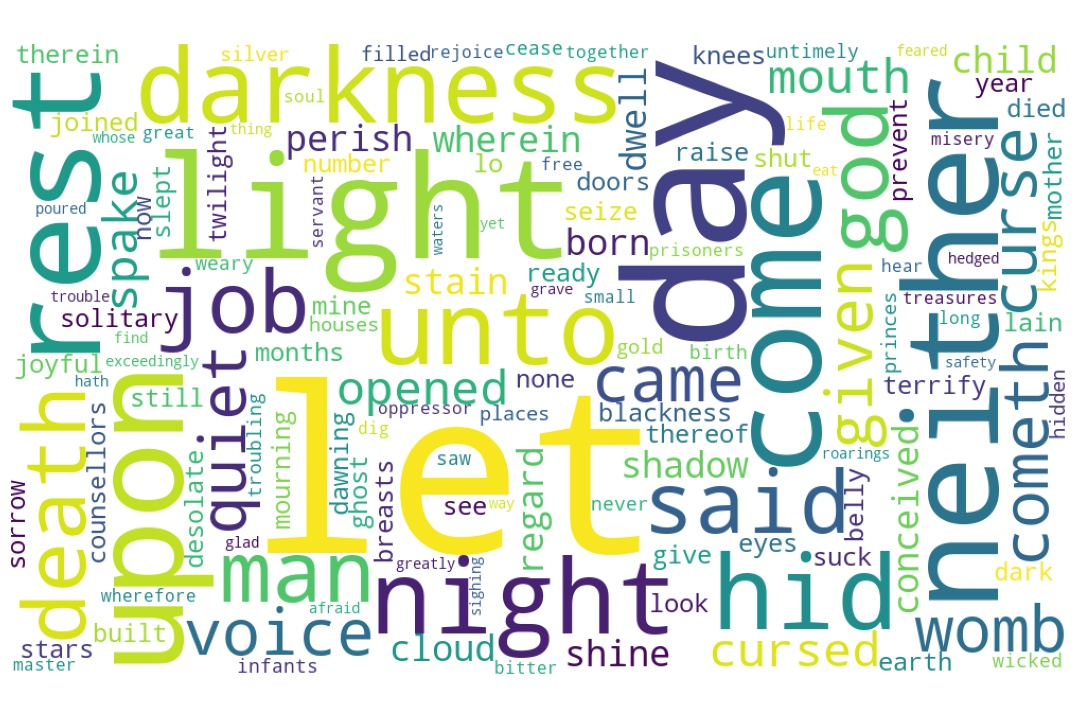
\includegraphics[width=\linewidth]{18OT-Job/Job003wordcloud.jpg}
  \caption{Job 3 Word Cloud}
  \label{fig:Job 3 Word Cloud}
\end{figure}




% [cmyk]{0.99998,1,0,0}{
% [cmyk]{0.99998,1,0,0}{

\marginpar{\scriptsize \centering \fcolorbox{bone}{lime}{\textbf{JOB'S QUESTION (PART I)}}\\ (Job 3:1-26) \begin{compactenum}[I.][8]
    \item  \textbf{Wherefore is light given} \index[scripture]{Job!Job 03:20}(Job 3:20)
    \item  \textbf{Why is light given to a man whose way is hid $\hdots$ ?} \index[scripture]{Job!Job 03:23}(Job 3:23)
    \item  \textbf{Shall mortal man be more just than God?} \index[scripture]{Job!Job 04:17}(Job 4:17)
    \item  \textbf{Shall a man be more pure than his maker?} \index[scripture]{Job!Job 04:17}(Job 4:17) 
    \item  \textbf{What is man that thou shouldest magnify him?} \index[scripture]{Job!Job 07:17}(Job 7:17)
    \item  \textbf{If I be wicked, why then labour I in vain?} \index[scripture]{Job!Job 09:29}(Job 9:29)
\end{compactenum}}


\marginpar{\scriptsize \centering \fcolorbox{bone}{yellow}{\textbf{JOB'S QUESTION (PART II)}}\\ (Job 3:1-26) \begin{compactenum}[I.][8]
    \item  \textbf{Canst thou by searching find out God?} \index[scripture]{Job!Job 11:07}(Job 11:7)
    \item  \textbf{Canst thou find out the Almighty unto perfection?} \index[scripture]{Job!Job 11:07}(Job 11:7)
    \item  \textbf{Man dieth, and wasteth away $\hdots$ and where is he?} \index[scripture]{Job!Job 14:10}(Job 14:10)
    \item  \textbf{What is man that he should be clean?} \index[scripture]{Job!Job 15:14}(Job 15:14)
    \item  \textbf{And he which is born of woman, that he should be righteous?} \index[scripture]{Job!Job 15:14}(Job 15:14)
    \item  \textbf{Wherefore do the wicked live?} \index[scripture]{Job!Job 21:7}(Job 21:7)
\end{compactenum}}

\marginpar{\scriptsize \centering \fcolorbox{bone}{black}{\textbf{\textcolor[cmyk]{0,0,0,0}{JOB'S QUESTION (PART III)}}}\\ (Job 3:1-26)  \begin{compactenum}[I.][8]
    \item  \textbf{Can a man be profitable unto God...?} \index[scripture]{Job!Job 22:02}(Job 22:2)
    \item  \textbf{How then can man be justified with God?} \index[scripture]{Job!Job 25:04}(Job 25:4)
    \item  \textbf{Whence then cometh wisdom? Where is $\hdots$understanding?} \index[scripture]{Job!Job 28:20}(Job 28:20)
    \item  \textbf{What profit shall I have if I be cleansed from my sin?} \index[scripture]{Job!Job 35:3}(Job 35:3)
    \item  \textbf{Where is God my maker $\hdots$?} \index[scripture]{Job!Job 35:10}(Job 35:10)
    \item  \textbf{Wilt thou condemn me, that thou mayest be righteous?} \index[scripture]{Job!Job 40:8}(Job 40:8)
    \item  \textbf{Who is he that hideth counsel without knowledge?} \index[scripture]{Job!Job 42:3}(Job 42:3)
\end{compactenum}}

\footnote{\textcolor[cmyk]{0.99998,1,0,0}{\hyperlink{TOC}{Return to end of Table of Contents.}}}\footnote{\href{https://www.audioverse.org/english/audiobibles/books/ENGKJV/O/Job/1}{\textcolor[cmyk]{0.99998,1,0,0}{Job  Audio}}}\textcolor[cmyk]{0.99998,1,0,0}{After this opened Job his mouth, and cursed his day.}
[2] \textcolor[cmyk]{0.99998,1,0,0}{And Job spake, and said,}
[3] \textcolor[cmyk]{0.99998,1,0,0}{Let the day perish wherein I was born, and the night \emph{in} \emph{which} it was said, There is a man child conceived.}\footnote{\textbf{Leviticus 12:1,2} - And the LORD spake unto Moses, saying, [2] Speak unto the children of Israel, saying, If a woman have conceived seed, and born a man child: then she shall be unclean seven days; according to the days of the separation for her infirmity shall she be unclean.}\footnote{\textbf{I Samuel 1:11} - And she vowed a vow, and said, O LORD of hosts, if thou wilt indeed look on the affliction of thine handmaid, and remember me, and not forget thine handmaid, but wilt give unto thine handmaid a man child, then I will give him unto the LORD all the days of his life, and there shall no razor come upon his head.}\footnote{\textbf{Isaiah 66:7,8} - Before she travailed, she brought forth; before her pain came, she was delivered of a man child. [8] Who hath heard such a thing? who hath seen such things? Shall the earth be made to bring forth in one day? or shall a nation be born at once? for as soon as Zion travailed, she brought forth her children.}\footnote{\textbf{Jeremiah 20:14-18} - Cursed be the day wherein I was born: let not the day wherein my mother bare me be blessed. [15] Cursed be the man who brought tidings to my father, saying, A man child is born unto thee; making him very glad. [16] And let that man be as the cities which the LORD overthrew, and repented not: and let him hear the cry in the morning, and the shouting at noontide; [17] Because he slew me not from the womb; or that my mother might have been my grave, and her womb to be always great with me. [18] Wherefore came I forth out of the womb to see labour and sorrow, that my days should be consumed with shame?}\footnote{\textbf{Revelation 12:5} - And she brought forth a man child, who was to rule all nations with a rod of iron: and her child was caught up unto God, and to his throne. 6 And the woman fled into the wilderness, where she hath a place prepared of God, that they should feed her there a thousand two hundred and threescore days.}\footnote{\textbf{Revelation 12:13} - And when the dragon saw that he was cast unto the earth, he persecuted the woman which brought forth the man child.}
[4] \textcolor[cmyk]{0.99998,1,0,0}{Let that day be darkness; let not God regard it from above, neither let the light shine upon it.}
[5] \textcolor[cmyk]{0.99998,1,0,0}{Let darkness and the shadow of death stain it; let a cloud dwell upon it; let the blackness of the day terrify it.}\footnote{\textbf{Isaiah 9:2} - The people that walked in darkness have seen a great light: they that dwell in the land of the shadow of death, upon them hath the light shined.}
[6] \textcolor[cmyk]{0.99998,1,0,0}{As \emph{for} that night, let darkness seize upon it; let it not be joined unto the days of the year, let it not come into the number of the months.}
[7] \textcolor[cmyk]{0.99998,1,0,0}{Lo, let that night be solitary, let no joyful voice come therein.}
[8] \textcolor[cmyk]{0.99998,1,0,0}{Let them curse it that curse the day, who are ready to raise up their mourning.}
[9] \textcolor[cmyk]{0.99998,1,0,0}{Let the stars of the twilight thereof be dark; let it look for light, but \emph{have} none; neither let it see the dawning of the day:}
[10] \textcolor[cmyk]{0.99998,1,0,0}{Because it shut not up the doors of my \emph{mother's} womb, nor hid sorrow from mine eyes.}
[11] \textcolor[cmyk]{0.99998,1,0,0}{Why died I not from the womb? \emph{why} did I \emph{not} give up the ghost when I came out of the belly?}
[12] \textcolor[cmyk]{0.99998,1,0,0}{Why did the knees prevent me? or why the breasts that I should suck?}
[13] \textcolor[cmyk]{0.99998,1,0,0}{For now should I have lain still and been quiet, I should have slept: then had I been at rest,}
[14] \textcolor[cmyk]{0.99998,1,0,0}{With kings and counsellors of the earth, which built desolate places for themselves;}
[15] \textcolor[cmyk]{0.99998,1,0,0}{Or with princes that had gold, who filled their houses with silver:}
[16] \textcolor[cmyk]{0.99998,1,0,0}{Or as an hidden untimely birth I had not been; as infants \emph{which} never saw light.}\footnote{\textbf{Psalm 58:8} - As a snail which melteth, let every one of them pass away: like the untimely birth of a woman, that they may not see the sun.}\footnote{\textbf{Ecclesiastes 6:3} - If a man beget an hundred children, and live many years, so that the days of his years be many, and his soul be not filled with good, and also that he have no burial; I say, that an untimely birth is better than he.}
\footnote{\textbf{Revelation 6:13} - And the stars of heaven fell unto the earth, even as a fig tree casteth her untimely figs, when she is shaken of a mighty wind.}\footnote{\textbf{1 Corinthians 15:8} - And last of all he was seen of me also, as of one born out of due time.}
[17] \textcolor[cmyk]{0.99998,1,0,0}{There the wicked cease \emph{from} troubling; and there the weary be at rest.}
[18] \textcolor[cmyk]{0.99998,1,0,0}{\emph{There} the prisoners rest together; they hear not the voice of the oppressor.}
[19] \textcolor[cmyk]{0.99998,1,0,0}{The small and great are there; and the servant \emph{is} free from his master.}
[20] \textcolor[cmyk]{0.99998,1,0,0}{Wherefore is light given to him that is in misery, and life unto the bitter \emph{in} soul;}
[21] \textcolor[cmyk]{0.99998,1,0,0}{Which long for death, but it \emph{cometh} not; and dig for it more than for hid treasures;}
[22] \textcolor[cmyk]{0.99998,1,0,0}{Which rejoice exceedingly, \emph{and} are glad, when they can find the grave?}
[23] \textcolor[cmyk]{0.99998,1,0,0}{\emph{Why} \emph{is} \emph{light} \emph{given} to a man whose way is hid, and whom God hath hedged in?}
[24] \textcolor[cmyk]{0.99998,1,0,0}{For my sighing cometh before I eat, and my roarings are poured out like the waters.}
[25] \textcolor[cmyk]{0.99998,1,0,0}{For the thing which I greatly feared is come upon me, and that which I was afraid of is come unto me.}
[26] \textcolor[cmyk]{0.99998,1,0,0}{I was not in safety, neither had I rest, neither was I quiet; yet trouble came.}